\documentclass{lebook}
\usepackage{lelists}
\setlength{\listtopsep}{0pt}
\setlength{\leftlistindent}{0pt}
\setlength{\rightlistindent}{0pt}

\usepackage{lefonts}
\usepackage{lefontsizes}
\usepackage{lecode}
\codefontsize{\small}

\usepackage{legraphicextensions}
\graphicspath{{Figures/}}

\usepackage{lesubscripts}
\usepackage[pdfauthor={Lance A. Endres}, pdftitle={WinEdt Installation Notes, colorlinks}]{lehyperlink}
\usepackage{leheadersandfooters}

\usepackage{leaddress}

\usepackage{times}

\newcommand{\tbs}{$\backslash$}
\newcommand*{\rootdir}{\textcode{\textit{root}}}
\newcommand*{\supportdir}{\textcode{\textit{support}}}
\newcommand*{\userdir}{\textcode{\textit{user}}}
\newcommand*{\plotstyledir}{\textcode{\textit{plotstyles}}}
\newcommand*{\templatedir}{\textcode{\textit{templates}}}

\newcommand*{\rootpath}{\rootdir\tbs}
\newcommand*{\supportpath}{\supportdir\tbs}
\newcommand*{\userpath}{\userdir\tbs}
\newcommand*{\plotstylepath}{\plotstyledir\tbs}
\newcommand*{\templatepath}{\templatedir\tbs}
%\newcommand*{}{}

%%%%%%%%%%%%%%%%%%%%%%%%%%%%%%%%%%%%%%%%%%%%%%%%%%%%%%%%%%%%%%%%%%%%%
% BEGIN DOCUMENT
%%%%%%%%%%%%%%%%%%%%%%%%%%%%%%%%%%%%%%%%%%%%%%%%%%%%%%%%%%%%%%%%%%%%%

\pagestyle{leplainheader}
\begin{document}

\chapter{Installation}
\section{Introduction}

\begin{tabular}{|l|l|}
  \hline
  % after \\: \hline or \cline{col1-col2} \cline{col3-col4} ...
  \rootdir & \textcode{C:\tbs{}Custom Program Files\tbs{}CAD Support Files\tbs{}} \\ \hline
  \supportdir & \rootpath\textcode{Support} \\ \hline
  \userdir & \rootpath\textcode{User Files} \\ \hline
  \plotstyledir & \rootpath\textcode{Plot Styles} \\ \hline
\end{tabular}


\section{Command Aliases (PGP)}
\begin{numberedlist}
    \item Open the software's PGP file.
    \item Copy of contents of the \userdir\tbs\textcode{user.pgp} to the bottom of the software's PGP file.
    \item Close the file and reload it.  The aliases at the bottom will override those at the top.
\end{numberedlist}

\section{Paths}
\begin{numberedlist}
    \item Open the options (command \textcode{options}).
    \item Add the support file path.
    \begin{numberedlist}
    	\item Expand \textcode{File$\rightarrow$Support File Search Path}.
    	\item Add the \supportdir{} directory.
    	\item Move the entry to the top so that anything in that directory is found first.  See \figurename~\ref{fig:addsupportdirectory}.
    \end{numberedlist}
    \item Add the plot style search path.
    \begin{numberedlist}
    	\item Expand \textcode{Printer Support File Path}$\rightarrow$\textcode{Plot Style Table Search Path}
    	\item Add the \plotstyledir{} directory.
    \end{numberedlist}
    \begin{numberedlist}
    	\item
    \end{numberedlist}
    \begin{numberedlist}
    	\item
    \end{numberedlist}
\end{numberedlist}

\begin{figure}
	\centering
	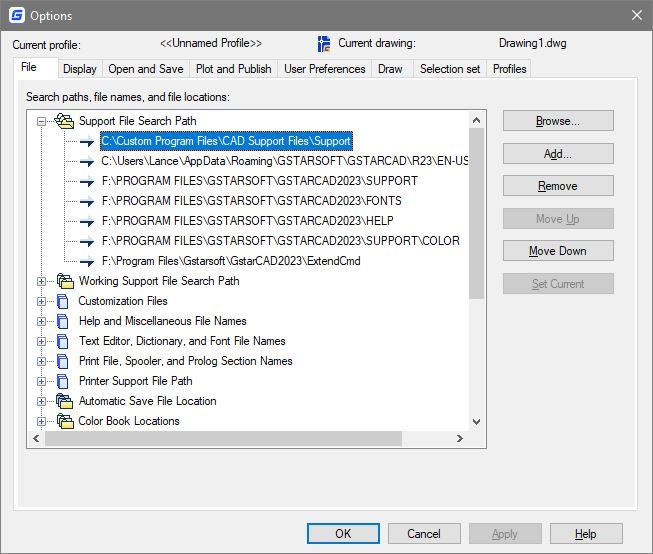
\includegraphics[width=3.25in]{addsupportdirectory}
	\caption{Add the user's support directory to the search path.}
	\label{fig:addsupportdirectory}
\end{figure}


\section{Lisp}
\begin{numberedlist}
    \item Find the software's \textcode{\textit{document}.lsp}.  Examples include:
    \begin{bulletedlist}
    	\item \textcode{acaddoc.lsp}
    	\item \textcode{gcad2023doc.lsp}.
    \end{bulletedlist}
    \item Copy it to the \supportdir{} directory.
    \item Edit the file to add the following the end (just before the file \textcode{(princ)} function):
    \begin{plainlist}
    	\item \textcode{; Added to support autoload of custom lisp files.}
		\item \textcode{(load "userdoc.lsp")}
    \end{plainlist}

\end{numberedlist}


%\begin{plainlist}
%	\item \textcode{BUTTON="Make\_Document"}
%\end{plainlist}


\chapter{Notes}
\begin{bulletedlist}
	\item \href{https://www.youtube.com/watch?v=Rrgx3TcXNzM}{Video on lisp debugging with GStar2023}
\end{bulletedlist}



\end{document} 